\documentclass[11pt]{article}
\usepackage[margin=1in]{geometry}
\usepackage{lmodern}
\usepackage[T1]{fontenc}
\usepackage{amsmath,amssymb}
\usepackage{booktabs}
\usepackage{graphicx}
\usepackage{url}
\setlength{\parskip}{0.4em}
\setlength{\parindent}{0pt}
\renewcommand{\arraystretch}{1.15}
\setlength{\tabcolsep}{4.5pt}

\title{\vspace{-1.2cm}\textbf{Replacing Transformer Feed-Forward Layers with Lookup Tables}}
\author{Anatoly Starostin \\ DeepSpike Inc.}
\date{Draft, \today}

\begin{document}
\maketitle
\vspace{-0.8cm}

\begin{abstract}
\noindent The feed-forward (FFN) sub-layer of a transformer is a dense two-layer MLP that accounts
for a large share of the model's per-token arithmetic and of the weight memory traffic read on
every token. We replace it with a family of lookup-table (LUT) designs and search through them for one that
matches the dense baseline's language-modelling quality at as small a parameter count as possible. In a sweep with each run
trained on about $400$ million tokens, these designs match or beat the dense baseline's bits per byte (bpb) at
comparable whole-model parameter count, while cutting the FFN block's per-token arithmetic by
roughly seven times and introducing a roughly sevenfold sparsity into its weight access that specialised
hardware could exploit and turn into further speedup. Three of the smallest configurations trained to
over one billion tokens stay within run-to-run noise of a matched dense
baseline, and a single representative tiny configuration taken much further, to about $3.5$ billion
tokens, still lands within run-to-run noise of the extended dense baseline,
so we treat them as equal in language-modelling quality. Because these models come so
close to the dense baseline in parameter count, we also measure the wall-clock speed of the FFN block directly on two GPUs: on an RTX~5090 the tiny LUT FFN runs $1.3$ to
$1.9$ times faster than the dense FFN, while on an H100 it is slightly slower,
because the H100's dense FFN is extremely fast on its tensor cores whereas the routing-and-gather
stage, which uses none, is bound by SM clock. We read that difference as indirect
evidence of the value of building specialised hardware for the lookup primitive. All
code is available at \url{https://github.com/anatoli-starostin/spiky}.
\end{abstract}

\section{Introduction}

Modern AI runs on dense matrix multiplication. Nearly every operation in a large language model is
a multiply-accumulate, and today's accelerators are built to run exactly that. It is easy to assume
this is fundamental, but it is largely an accident of hardware. As set out in the Spiking
Manifesto~\cite{manifesto}, dense matrix multiplication came to dominate deep learning because it
won the GPU hardware lottery: GPUs happened to be good at it, so the whole field leaned into the
operation the available hardware ran fastest.

The object of interest in this work is a single computational primitive, the lookup table,
introduced in the Spiking Manifesto~\cite{manifesto}. The idea is not raw storage but conditional retrieval: we keep a large number of parameters, and
each input is hashed by a handful of cheap comparisons into an address that selects the small
fraction of them to read out and combine. The basic operation is this input-dependent lookup,
storage and routed retrieval, rather than multiply-accumulate. We make no strong claim about biology,
and the primitive need not even be read as brain-inspired. But we think it is a good abstraction of
the kind of computation that real spiking networks carry out.

From this high-level idea we descend to a concrete problem, and the obvious choice is language
modeling. Decoder-only language models trained to predict the next token are the dominant paradigm
in modern deep learning, and they sit at the core of the systems people use every day, such as ChatGPT, Claude,
and Gemini. Next-token prediction has come to be seen as a genuinely fundamental task, one that
scales into broad capability. So if we are going to propose something as large as replacing matrix
multiplication, even partially, we have to show that it works on the central problem of the field,
autoregressive language modeling.

In this paper we ask whether the feed-forward layers of a
transformer can be built from lookup tables instead of dense matrix multiplication, without loss of
language-modeling quality.

Our setup is deliberately ordinary. We build on Andrej Karpathy's nanochat~\cite{nanochat}, a
publicly available language-modeling framework positioned as a sandbox for researchers who want to
understand language modeling at the GPT-2 level. GPT-2 is not a simple model, but it is well suited
to scientific work: it is small enough to fit on a single GPU, so experiments are cheap to run and
to reproduce. The nanochat project has become a well-known entry point for researchers beginning in
language modeling, so choosing it as our starting point was a logical rather than an arbitrary decision. From it we
take the training setup, including the data and tokenization. As our baseline we deliberately use a
model even simpler than the one that ships with nanochat; it is still enough to reach good quality,
as we justify later in the paper. Concretely, the model is a decoder-only transformer with six
layers, model dimension $d=384$, feed-forward hidden size $4d=1536$, and context length $512$; the
dense baseline has $35.79$M parameters.

The rest of the paper is organized as follows. We first present the cost metrics we use to compare
designs. We then fix a vanilla dense baseline and, through a
series of experiments, try a progression of lookup-table designs for its feed-forward layers,
refining the architecture step by step until we reach one that recovers the baseline's
language-modeling quality at as low a parameter count as possible. We check that the match holds at a longer training horizon, and we finish by measuring the
efficiency of the lookup block on real GPUs.

\section{Reported metrics}

The dense FFN multiplies and reads every one of its weights on every token, with an inner widening
to $4d$. A lookup-table block is sparse by construction: each token is routed with a handful of
cheap comparisons, and only a small number of stored rows are read and summed, with no large matrix
multiply. This cuts both arithmetic and memory traffic, at the price of storing many table rows.
Our two cost metrics are designed to capture this dense-versus-sparse contrast, one for arithmetic
and one for memory.

We report two cost metrics for every run, and \textbf{both are for the FFN block alone},
per token, not the whole model. Attention and the unembedder are identical across every
variant (only the FFN is replaced), so the FFN-block figures are what isolate the effect
of the replacement; whole-model figures would merely add the same constant to every row.
Our baseline has only six layers and is dominated by the unembedder, so at the whole-model
level the FFN saving is diluted; but the model is big enough for our study: it reaches low
perplexity without spending too much compute.\footnote{A byte-level bpb of about 1.2 at
context 512 is far below what trivial baselines achieve: general-purpose compressors and
low-order n-gram models over natural-language bytes land substantially higher: gzip
reaches only about 2.9 bits per byte on the standard enwik8 text benchmark~\cite{ltcb}, and
low-order byte n-gram models remain above 2 bits per byte. Reaching about 1.2 bpb is
therefore a genuine modeling regime that exercises the network's (and hence the FFN's)
real capacity, not a toy task.}
\textbf{FLOPs} is the per-token forward arithmetic of the FFN block:
the input reprojection and output decompression matmuls, if present (each multiply-add is two
FLOPs), plus one FLOP for each anchor comparison and one FLOP for each addition in the
gather-and-sum. The index selection itself is a gather, not a multiplication, and is treated as
precomputed at deployment, so it adds nothing beyond those comparisons and sums. A dense MLP FFN,
having no routing, is just its two matmuls.
\textbf{Virtual bandwidth} (vBW) is the FFN-block weight-and-activation memory traffic per
token in the single-token (decode) regime, in bytes: dense FFN weights (reprojection and
decompression matrices) read in full, LUT tables read as \emph{selected rows only}.\footnote{This
saving is clearest in single-token decoding, the batch-size-one regime that vBW measures: each
token reads only the rows its routing selects. This regime is not hypothetical: it is exactly how
on-device and edge generation run, decoding tokens one at a time at batch size one after the prompt
has been ingested. At large batch sizes different tokens select
different rows, so across a batch the union of accessed rows can approach the full weight set and
the per-token advantage shrinks. We nonetheless report vBW because the sparsity it captures is a
real structural property that suitable hardware could exploit; the resulting benefit is not a fixed
factor but depends on the batch size, on how much the selected rows overlap across tokens, and on
structural properties of the hardware.} The
"selected rows only" assumption is a property of specialised hardware, a gather that
touches one row per table rather than streaming the whole table. On commodity hardware the
full table is read; vBW is therefore the figure a LUT-aware accelerator would achieve, and we
label it accordingly. All bpb are validation bits per byte; lower is
better.

\section{Vanilla baseline}

The reference model is a decoder-only transformer: six layers, model dimension $d=384$, six
attention heads, rotary positional encodings, vocabulary $32{,}768$, sequence length $512$, and an
\emph{untied} unembedder (a separate output projection, not sharing the token-embedding
matrix). The FFN is the standard dense MLP: two linear layers with an inner widening to $4d$
and a GELU nonlinearity between them, $\mathrm{FFN}(x)=W_2\,\sigma(W_1 x)$ with
$W_1\in\mathbb{R}^{4d\times d}$ and $W_2\in\mathbb{R}^{d\times 4d}$. This is the baseline every
LUT variant is compared against, at equal training budget.

From nanochat~\cite{nanochat} we adopt the training setup: the ClimbMix dataset, the byte-pair
tokeniser and its $32{,}768$-token vocabulary, and the $512$-token context length that nanochat
uses for its short runs (not its full context). Unless noted, runs train for $16{,}000$ steps at
a batch of $48$ sequences of length $512$ ($24{,}576$ tokens total), so that comparisons across
variants hold the data and the compute budget fixed and vary only the FFN.

The optimiser is AdamW with $\beta=(0.9,0.95)$, $\epsilon=10^{-8}$, and peak learning rate
$3\times10^{-4}$. Weight decay is $0.1$ on the two-dimensional weight matrices and $0$ on the
LUT tables, the LUT temperatures, and all one-dimensional parameters (biases and norms). The
learning rate follows a linear warmup over the first $10\%$ of the schedule ($1{,}600$ steps
for the $16{,}000$-step runs) and a cosine decay thereafter to $0.1\times$ the peak
($3\times10^{-5}$).

\begin{table}[h]\centering
\begin{tabular}{lrrr}
\toprule
run & bpb & FLOPs/tok & vBW/tok \\
\midrule
exp\_n\_0135 (vanilla) & 1.20144 & 14.16M & 14.16M \\
\bottomrule
\end{tabular}
\caption{Vanilla baseline; FLOPs/vBW are the dense MLP FFN block. Parameters: 35.79M whole-model.}
\end{table}

\section{Straightforward FFN $\rightarrow$ LUT replacement}
\label{sec:straightforward}

\paragraph{Construction (forward).} We replace each transformer layer's FFN by a multi-table
lookup layer of the Spiking-Manifesto form~\cite{manifesto}. The layer holds $R$ tables.
Each table $t$ owns $k$ \emph{anchor pairs} $(a_{tj},b_{tj})_{j=1}^{k}$ (pairs of input
coordinates fixed at construction) and a weight bank $W_t\in\mathbb{R}^{2^{k}\times d}$ of
$2^{k}$ stored rows of width $d$. For an input $x\in\mathbb{R}^{d}$, table $t$ runs its $k$
anchor comparisons, packs their outcomes into a $k$-bit integer index, and selects the
corresponding row:
\begin{equation}
\mathrm{idx}_t(x)=\sum_{j=1}^{k} 2^{\,j-1}\,\mathbf{1}\!\left[x_{a_{tj}}>x_{b_{tj}}\right]
\;\in\;\{0,\dots,2^{k}-1\}.
\end{equation}
The layer output is the sum of the selected rows over all tables, an embedding-bag
reduction:
\begin{equation}
\mathrm{LUT}(x)=\sum_{t=1}^{R} W_t\!\left[\,\mathrm{idx}_t(x)\,\right].
\end{equation}
The forward pass performs \emph{no multiplications}: $k$ comparisons and a bit-pack per table
produce the index, and a gather-and-add produces the output. The index computation is the
routing; the stored rows are the parameters.

\paragraph{Backward (hard forward, soft backward).} The index is a step function of $x$ and
is not differentiable, so training uses a soft surrogate: the forward value is the hard
selection above, while the backward pass differentiates a soft distribution over all $2^{k}$
rows of each table. The surrogate carries two learnable temperatures per table, $T_{\mathrm{soft}}$
and $T_{\mathrm{sel}}$. For table $t$ let $d_{j}=x_{a_{tj}}-x_{b_{tj}}$ be the signed margin of
anchor $j$. Each margin is relaxed by a \emph{rational soft-sign} at temperature $T_{\mathrm{soft}}$,
\begin{equation}
p_{j}\;=\;\frac{d_{j}}{\,T_{\mathrm{soft}}+|d_{j}|\,}\;=\;\operatorname{sign}(d_{j})\,\frac{|d_{j}|}{\,T_{\mathrm{soft}}+|d_{j}|\,}\;\in(-1,1),
\qquad
\frac{\partial p_{j}}{\partial d_{j}}=\frac{T_{\mathrm{soft}}}{(T_{\mathrm{soft}}+|d_{j}|)^{2}} .
\end{equation}
Each candidate row $b\in\{0,1\}^{k}$ is scored by the agreement of its bit pattern with the
soft margins, $z_{b}=\sum_{j=1}^{k} \sigma_{jb}\,p_{j}$ with $\sigma_{jb}=2\,b_{j}-1\in\{-1,+1\}$,
and the rows are given a full-$K$ softmax at the \emph{selection} temperature $T_{\mathrm{sel}}$,
\begin{equation}
\pi_{b}\;=\;\frac{\exp(z_{b}/T_{\mathrm{sel}})}{\sum_{b'}\exp(z_{b'}/T_{\mathrm{sel}})} ,
\end{equation}
pinned so that $\arg\max_{b}\pi_{b}$ equals the row selected in the forward pass. So
$T_{\mathrm{soft}}$ sets the sharpness of each per-anchor comparison and $T_{\mathrm{sel}}$
the sharpness of the row distribution; both are learnable and both receive gradient in this
hard-forward backward. The two gradient paths are distinct. The weights are updated only
through the hard forward pick: only the selected row's weights receive the upstream gradient;
the other $2^{k}-1$ rows of the table are untouched. The full-$K$ softmax exists solely as the
surrogate that carries gradient to the \emph{routing} (the input $x$ and the two
temperatures $T_{\mathrm{soft}}$, $T_{\mathrm{sel}}$) through the softmax Jacobian
$\partial z_{b}=\pi_{b}\big(g_{b}-\sum_{b'}\pi_{b'}g_{b'}\big)$ (which yields the
$T_{\mathrm{sel}}$ gradient directly) composed with $\partial p_{j}/\partial d_{j}$ above for
$x$ and $T_{\mathrm{soft}}$, where $g_{b}=\langle\text{upstream},\,W_t[b]\rangle$. So the soft
distribution moves the anchors and both temperatures, while the weights of one row per table
are learned by ordinary supervision on the selected row.

\paragraph{Result.} A direct replacement reaches baseline bpb, but only with a large table
budget: to match the vanilla bpb it must store many wide rows. The bpb-matched configuration
(Table~2) uses $R=512$ tables with $k=8$ anchor-pair
comparisons per table ($2^{8}=256$ rows of width $d$ each), and attains $1.20567$ (within
$0.004$ of the vanilla $1.20144$) but at
$330.7$M parameters, roughly $9\times$ the whole-model parameter count of the baseline and
about $43\times$ the parameters of the dense FFN it replaces. FLOPs and virtual bandwidth
are already favourable: with the routing gather replacing both dense matmuls, the FFN block has
no matmul, and its per-token arithmetic falls to $\approx 1.20$M FLOPs (entirely the anchor
comparisons and the gather-sum over the wide rows) and $\approx 2.36$M bytes per token, against
the dense FFN's $14.16$M and $14.16$M.

\begin{table}[h]\centering
\begin{tabular}{lrrr}
\toprule
run & bpb & FLOPs/tok & vBW/tok \\
\midrule
exp\_n\_0136 (straightforward LUT; $R{=}512$, $k8$) & 1.20567 & 1.20M & 2.36M \\
\bottomrule
\end{tabular}
\caption{Straightforward LUT replacement, bpb-matched; FFN-block FLOPs/vBW (pure table
gather, no matmul). Parameters: 330.7M whole-model (naive footprint).}
\end{table}

\section{Output compression}
\label{sec:compression}

We have already established a LUT model that beats the dense baseline on both FLOPs and virtual
bandwidth, and such a model could be deployed given some form of hardware LUT
accelerator. It is nonetheless worth reducing the LUT parameter count while holding bpb fixed,
because a smaller table budget could in principle allow LUT models to run on ordinary GPUs.
A second reason is training time: the soft backward materialises a distribution over all
$2^{k}$ rows of every table, so its cost scales with the table budget, and larger LUT models
are correspondingly slower to train in wall-clock terms, so reducing the parameter count
shortens training as well. The remainder of the paper pursues this goal: to find more compact
LUT architectures that, relative to the vanilla baseline, are better in FLOPs and virtual
bandwidth and equal or better in bpb.

First we try to attack the table rows directly: we let them emit a \emph{compressed}
output of width $c<d$, and restore full width with a small learned matrix
$D\in\mathbb{R}^{d\times c}$: $\mathrm{FFN}(x)=D\,\mathrm{LUT}_c(x)$. This introduces one
matmul ($c\!\to\!d$, far smaller than the dense FFN's two $d\!\to\!4d$ matmuls) but shrinks
every stored row from $d$ to $c$. We also split the layer into $H$ heads; every head reads the
whole input (its tables anchor over all $d$ coordinates, not a private slice), and the
split is on the output side: each head emits its own $c$-wide compressed output ($c=48$,
restored to the full width $d=384$), and these are
concatenated before the single decompression. Output compression alone (no input-side change)
cuts the footprint by roughly $5\times$ against the straightforward replacement, at a small
bpb cost.

\begin{table}[h]\centering
\begin{tabular}{lrrr}
\toprule
run & bpb & FLOPs/tok & vBW/tok \\
\midrule
exp\_n\_0138 (output-compress only) & 1.21249 & 1.06M & 1.18M \\
\bottomrule
\end{tabular}
\caption{Output compression only ($H4$, $k=8$, tph128, $c=48$). Parameters: 66.9M, a $\sim$5$\times$ footprint reduction vs.\ Section~\ref{sec:straightforward} for $+0.007$ bpb.}
\end{table}

\section{LUTs with input reprojection}

Output compression shrank the footprint but regressed quality: the compressed model of
Section~\ref{sec:compression} reached only $1.21249$ bpb, above the $1.20144$ baseline. We looked for a way to
recover quality without giving back the parameter savings.

The route we found is on the input side. Anchor-pair routing is more effective when the
tested coordinates live in a small subspace (random anchor pairs discriminate better in
low dimension), so we \emph{reproject} the input into a small dimension $d_{\mathrm{in}}$
with a learned matrix before the comparisons, and route within that subspace. The reprojection
reduces the number and width of tables needed to cover the input, and the added input matmul
is still far below the dense FFN cost, so FLOPs and virtual bandwidth remain favourable.

This recovered the quality. We found a configuration, exp\_n\_0121, with substantially better
bpb than output compression and below the baseline: $67.4$M parameters, bpb $1.19142$, and an
FFN block of $1.94$M FLOPs and $2.07$M virtual bandwidth per token.

Having found this configuration, we were curious about its neighbourhood, so we swept
hyperparameters around it: the number of anchor pair comparisons $k$, tables per head, head count, and reprojection
width. Table~4 reports the sweep (exp\_n\_0121 marked $\ast$). Several configurations beat the
vanilla baseline at or below its bpb; the depth and table-count axes trade bpb for parameters
near-monotonically, while the head/reprojection split at fixed budget is close to flat. The
best on-budget points reach bpb $1.179$--$1.189$ at $67$--$181$M parameters.

\begin{table}[h]\centering
\begin{tabular}{lrrl}
\toprule
run & bpb & params & FLOPs/tok \,/\, vBW/tok \\
\midrule
exp\_n\_0135 (vanilla baseline) & 1.20144 & 35.79M & 14.16M / 14.16M \\
exp\_n\_0126 ($H4d48$, $k7$, tph64) & 1.20694 & 39.0M & 1.85M / 1.92M \\
exp\_n\_0153 ($H2d96$, $k7$, tph64) & 1.20772 & 39.0M & 1.85M / 1.92M \\
exp\_n\_0128 ($H4d48$, $k8$, tph64) & 1.20228 & 48.5M & 1.86M / 1.92M \\
exp\_n\_0127 ($H4d48$, $k7$, tph128) & 1.19471 & 48.5M & 1.94M / 2.07M \\
exp\_n\_0084 ($H4$, reprojection) & 1.19866 & 67.4M & 2.11M / 2.37M \\
exp\_n\_0137 ($H1d192$, $k8$, tph128) & 1.19432 & 67.4M & 1.92M / 2.07M \\
exp\_n\_0132 ($H8d24$, $k8$, tph128) & 1.19263 & 67.4M & 1.97M / 2.07M \\
exp\_n\_0121 ($H4$, $k8$, tph128) $\ast$ & 1.19142 & 67.4M & 1.94M / 2.07M \\
exp\_n\_0131 ($H2d96$, $k8$, tph128) & 1.18883 & 67.4M & 1.93M / 2.07M \\
exp\_n\_0130 ($H4d48$, $k10$, tph64) & 1.19363 & 105.1M & 1.86M / 1.92M \\
exp\_n\_0119 ($k9$, tph128) & 1.18386 & 105.1M & 1.95M / 2.07M \\
exp\_n\_0129 ($H4d48$, $k8$, tph256) & 1.18074 & 105.1M & 2.11M / 2.37M \\
exp\_n\_0118 ($k9$, full) & 1.17431 & 180.6M & 2.12M / 2.37M \\
exp\_n\_0133 ($H4d48$, $k10$, tph128) & 1.17910 & 180.6M & 1.95M / 2.07M \\
\bottomrule
\end{tabular}
\caption{Input-reprojection sweep around anchor exp\_n\_0121 ($\ast$). The runs bracket the
vanilla bpb (the best well below it, a few of the smallest above) while the FFN block costs
$\sim$7$\times$ fewer FLOPs ($\approx$1.9--2.1M vs.\ the dense FFN's $14.16$M) and $\sim$6--7$\times$ less
virtual bandwidth ($\sim$2M vs.\ $14.16$M); the cost is parameters.}
\end{table}

Figure~\ref{fig:16k} places every run on the bpb--parameter plane against the vanilla baseline
($35.79$M, bpb $1.20144$). Most input-reprojection configurations fall below the baseline; the
frontier reaches bpb $1.17431$ at $180.6$M (exp\_n\_0118), while the smallest configurations, the
straightforward replacement ($1.20567$), and output compression ($1.21249$) sit above it.
Parameter budget is the axis along which the families separate.

\begin{figure}[p]\centering
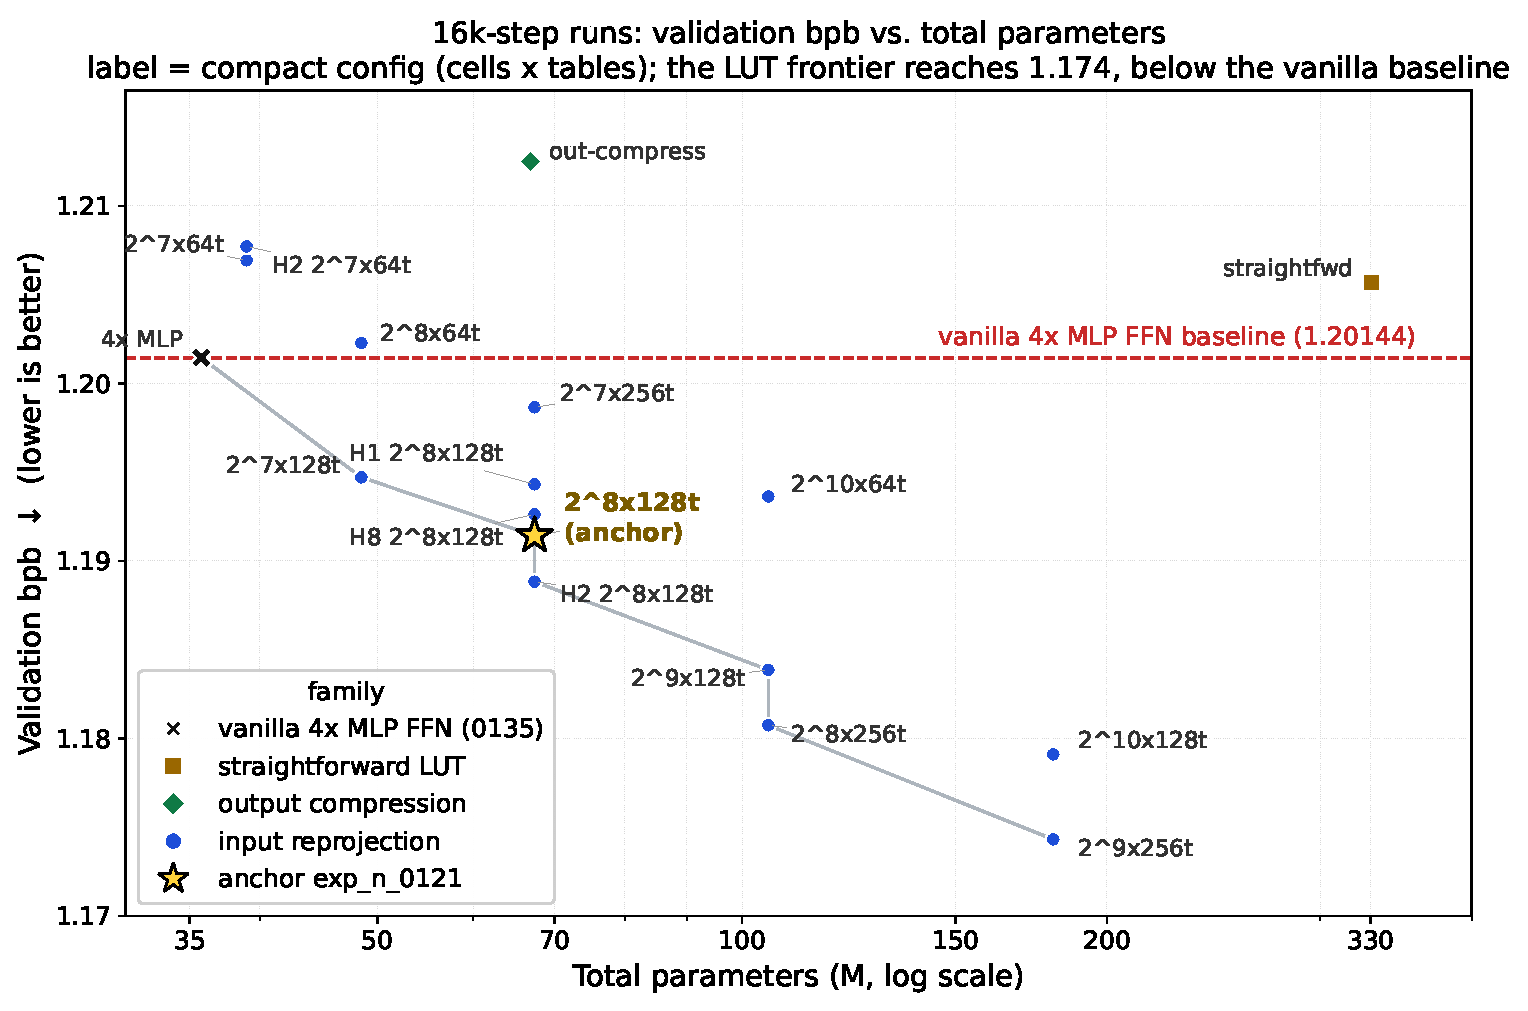
\includegraphics[width=0.95\linewidth]{fig16k.pdf}
\caption{Validation bpb against total parameters (log scale) for all 16k-step runs. Each marker
carries a compact config tag, cells$\times$tables ($2^{\mathrm{nap}}\times\mathrm{tph}$) for
the routed points. The red dashed line is the vanilla baseline ($1.20144$), the gold star is the
reprojection anchor exp\_n\_0121, and the grey line is the Pareto frontier, which reaches
$1.17431$ at $180.6$M (exp\_n\_0118); straightforward replacement and output compression sit
above the baseline. Lower is better.}
\label{fig:16k}
\end{figure}

Figure~\ref{fig:grid} resolves the reprojection sweep along two further axes: (a) validation bpb
against FFN virtual bandwidth for the higher-table iso-parameter families (more tables lower
bpb but raise bandwidth), and (b) the head sweep at fixed budget ($H\!\cdot\!d=192$,
$2^{8}\times128$ tables), where fewer, wider heads win and the anchor exp\_n\_0121 is the $H4$
point.

\begin{figure}[p]\centering
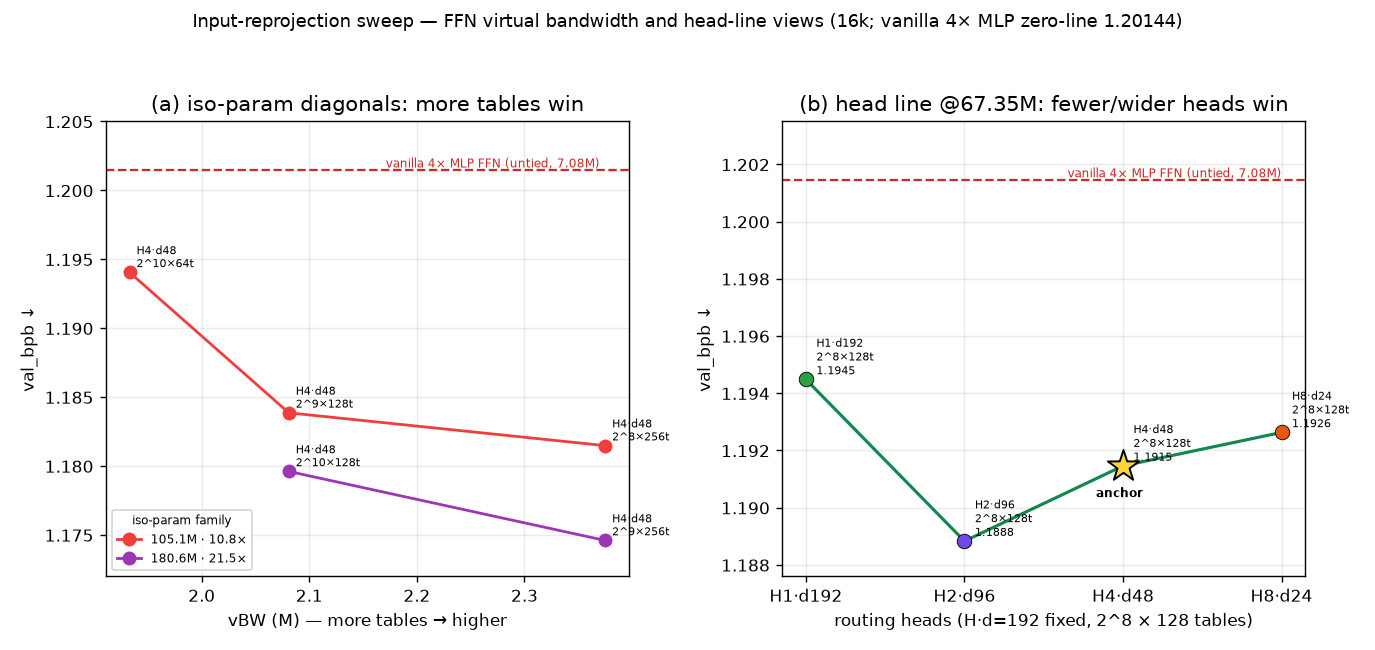
\includegraphics[width=0.95\linewidth]{FFN_GRID_plots.png}
\caption{Input-reprojection sweep, two views (zero-line = vanilla FFN, exp\_n\_0135,
$1.20144$ bpb). (a) bpb against FFN virtual bandwidth for the higher-table families; (b) the head
sweep at fixed budget, with the anchor exp\_n\_0121 as the gold star. Lower is better on both bpb
axes.}
\label{fig:grid}
\end{figure}

\clearpage
\section{Tiny LUT models at a longer horizon}

The aim of the reprojection sweep was not only to match the vanilla baseline's bpb but to do so
with the fewest parameters. Among the configurations that reach baseline quality with fewer
multiplications and lower virtual bandwidth, the interesting ones are the smallest, and several
are surprisingly small, close to the baseline's whole-model parameter count, the smallest
within about a tenth of it ($39.0$M against $35.79$M).

\paragraph{Longer-training check.} A model that matches at $16$k steps might still converge worse
over a longer horizon. To rule this out we took three of the smallest reprojection LUT
configurations and trained each on over one billion tokens ($48{,}000$ steps, batch $24{,}576$
tokens), alongside a matched long vanilla baseline (Table~\ref{tab:long}, Figure~\ref{fig:long}).
At this horizon the
tiny LUT models stay within noise of the vanilla baseline ($1.15602$, $1.15793$, and $1.15962$
against $1.15144$, comfortably within run-to-run variation), so we treat them as
equivalent to the baseline in language-modelling quality.

\begin{table}[h]\centering
{\small
\begin{tabular}{llrrl}
\toprule
run & config & bpb & params & FFN FLOPs\,/\,vBW \\
\midrule
exp\_n\_0151 & vanilla dense MLP & 1.15144 & 35.79M & 14.16M / 14.16M \\
exp\_n\_0152 (exp\_n\_0126 architecture) & $H4d48$, $k7$, tph64 & 1.15962 & 39.04M & $\approx$1.85M / $\approx$1.92M \\
exp\_n\_0155 (exp\_n\_0127 architecture) & $H4d48$, $k7$, tph128 & 1.15602 & 48.48M & $\approx$1.94M / $\approx$2.07M \\
exp\_n\_0156 (exp\_n\_0128 architecture) & $H4d48$, $k8$, tph64 & 1.15793 & 48.48M & $\approx$1.86M / $\approx$1.92M \\
\bottomrule
\end{tabular}
}
\caption{Long runs ($48{,}000$ steps, over $1$B tokens). The tiny reprojection LUT models match
the long vanilla baseline in bpb. FFN FLOPs/vBW are the deployed-basis reprojection costs derived
from each config (the $16$k grid points $0126$, $0127$, $0128$).}
\label{tab:long}
\end{table}

\begin{figure}[h]\centering
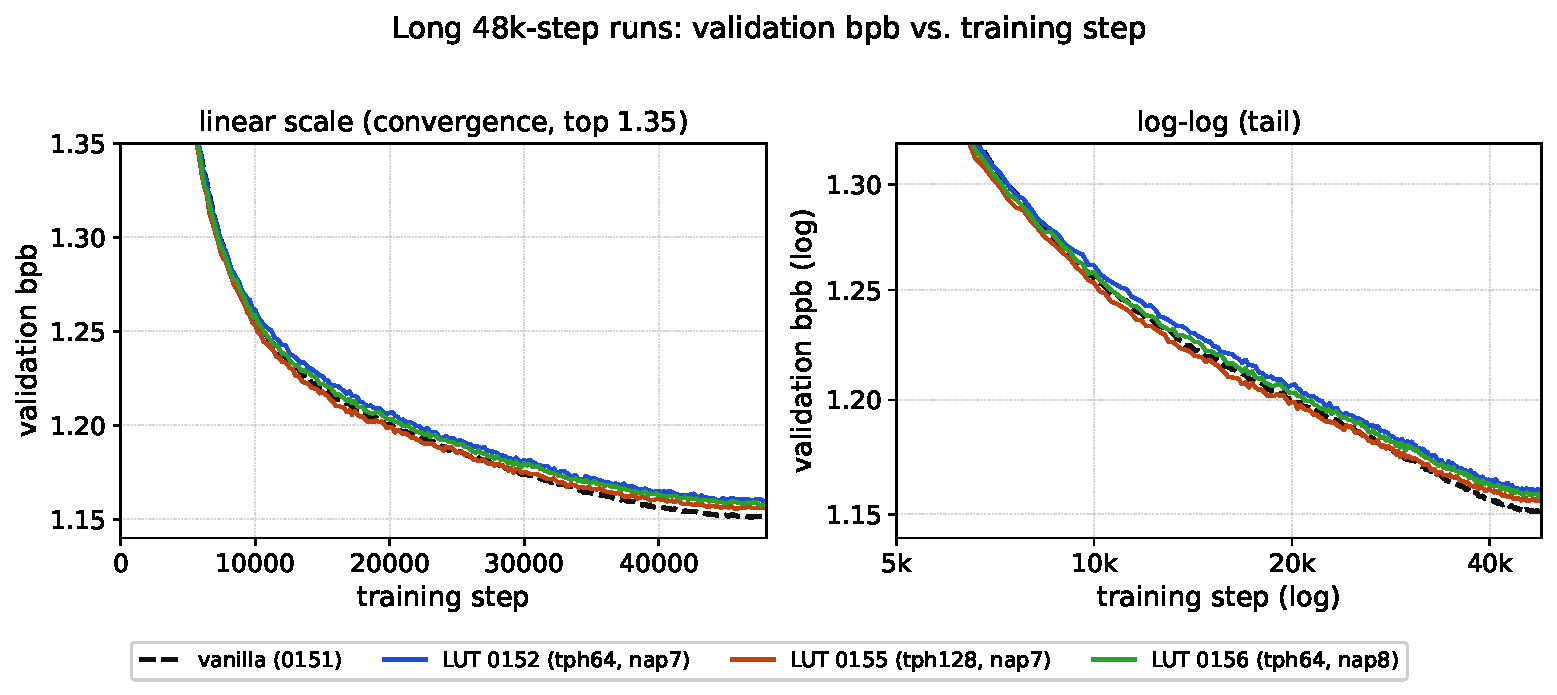
\includegraphics[width=\linewidth]{long_runs_fig.pdf}
\caption{Validation bpb against training step for the long $48{,}000$-step runs, a convergence
view (linear, top $1.35$; the early transient runs off the top) and a log--log view of the tail.
The three tiny reprojection LUT runs (exp\_n\_0152, exp\_n\_0155, exp\_n\_0156) track the vanilla
dense-MLP baseline (exp\_n\_0151, dashed) closely, with a small consistent offset (final bpb
$1.1560$, $1.1579$, $1.1596$ against $1.1514$).}
\label{fig:long}
\end{figure}

\paragraph{Super-long run.} The $48{,}000$-step runs above are the middle-length check. Runs
several times longer are expensive in GPU hours, so to be sure the match holds at a genuinely long
horizon we took a single representative tiny configuration, the exp\_n\_0127 architecture
($H4d48$, $k7$, tph128, $48.48$M parameters), and trained it far past the grid, to $144{,}000$
steps (about $3.5$ billion tokens at batch $24{,}576$). To keep the comparison apples-to-apples we
extended the vanilla baseline to the same length. At $144{,}000$ steps the LUT model reaches
$1.148013$ bpb against the vanilla baseline's $1.147985$, a difference of $0.000028$ bpb, far
inside run-to-run noise. The two curves track each other throughout (Figure~\ref{fig:superlong}):
the vanilla model leads during the early warmup, the curves cross near step $8{,}000$, the LUT sits
a hair ahead through the middle of training, and they re-converge at the end. At about $3.5$
billion tokens the tiny reprojection LUT still lands right on top of the dense baseline, with no
late-horizon divergence.\footnote{Training lookup tables is quite different from training a dense
MLP. The routing is built from hard sign comparisons, so it is not differentiable as
written; we train it with surrogate gradients (a hard forward pass with a soft, temperature-scaled
backward pass), and it took considerable experimentation to get it to train stably and match the
dense baseline. We regard how best to train such models, and how to do so most efficiently, as an
open problem. In particular they may benefit from optimizers other than Adam and from
learning-rate schedules different from those that are standard for dense transformers.}

For both the middle-length and the super-long runs the learning-rate schedule is rescaled to the
run length rather than reused from the $16$k grid: a linear warmup over the first $10\%$ of steps
followed by a cosine decay to zero across the full horizon (warmup $4{,}800$ then cosine to
$48{,}000$ for the middle-length runs, and warmup $14{,}400$ then cosine to $144{,}000$ for the
super-long run).

\begin{figure}[h]\centering
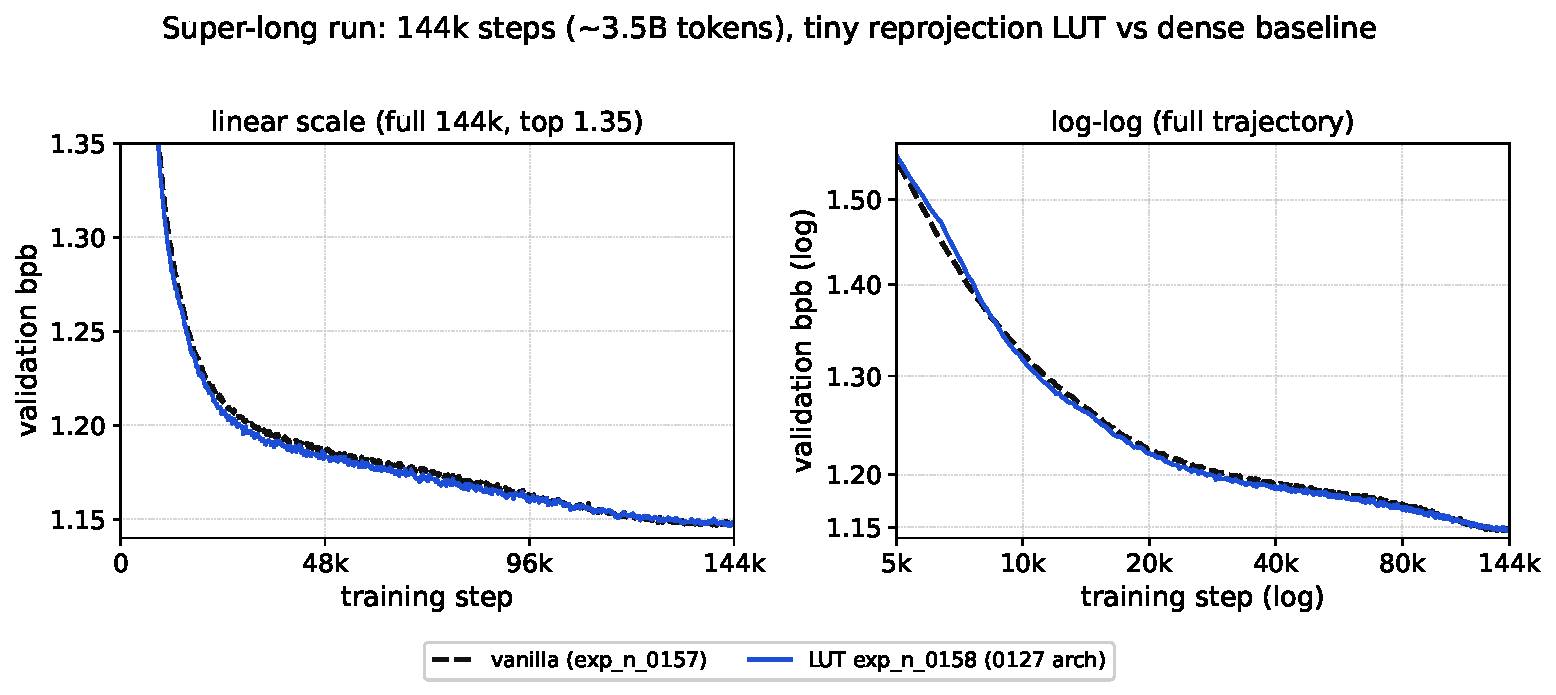
\includegraphics[width=\linewidth]{superlong_fig.pdf}
\caption{Validation bpb against training step for the super-long $144{,}000$-step run (about
$3.5$B tokens): the tiny reprojection LUT (exp\_n\_0158, the exp\_n\_0127 architecture) against the
matched vanilla dense baseline (exp\_n\_0157, dashed), extended to the same length. Left, the full
horizon on a linear scale framed at top $1.35$; right, a log-log view of the full trajectory. The
two curves sit on top of each other, ending at $1.148013$ and $1.147985$ bpb, a $0.000028$ bpb
difference.}
\label{fig:superlong}
\end{figure}

\clearpage
\section{Efficiency on GPUs}
\label{sec:gpu}

The tiny reprojection LUT models are small enough that it becomes worth measuring their inference
speed on standard modern GPUs directly. For larger LUT models the answer is known in advance: on commodity hardware,
which reads the whole table rather than only the selected rows, they are slower than the dense FFN,
and only the specialised hardware assumed for the virtual-bandwidth accounting above would change
that. The tiny reprojection LUTs are the case where the outcome is not obvious, so we measure it,
benchmarking the FFN slot on two cards, an RTX~5090 and an H100.

\paragraph{Method.} Modern GPUs are heavily optimised for matrix multiplication (GEMM) but offer
no comparable acceleration for the gather/lookup path, so the only lever is hand-written CUDA. We
applied extensive micro-optimisation (fused routing-and-gather kernels, shared-memory staging
of the index, conflict-free layouts), tuned separately for each card. The detailed kernel and
optimisation description is deferred to a later revision; here we report the timings.

\paragraph{Results.} Table~\ref{tab:bench} gives the FFN-slot time per call (batch $48$ sequences
$\times512$ tokens $=24{,}576$ tokens, bf16, warmed, \texttt{no\_grad}); Figure~\ref{fig:bench}
breaks it down by stage on the two cards. On the RTX~5090 the tiny LUT FFN
is $1.27$--$1.91\times$ faster than the vanilla dense FFN at identical language-modelling quality,
a clear win. On the H100 the same models are slightly slower (LUT/vanilla $1.108$--$1.833$),
because the H100's dense FFN is extremely fast on its tensor cores ($0.153$ ms per call), while
the routing and gather goes the opposite way and is slower on the H100, being bound by SM clock
rather than tensor cores; the gap for the tph64 configs is only $11$--$15\%$, but the fused kernel
does not overtake.

\begin{table}[h]\centering
\begin{tabular}{lrr}
\toprule
run (config) & RTX~5090: ms/call (speedup) & H100: ms/call (LUT$/$vanilla) \\
\midrule
vanilla dense MLP           & 0.34288 (1.00$\times$) & 0.153 (1.00$\times$) \\
exp\_n\_0126 ($k7$, tph64)  & 0.17984 (1.91$\times$) & 0.16890 (1.108$\times$) \\
exp\_n\_0128 ($k8$, tph64)  & 0.18752 (1.83$\times$) & 0.17560 (1.152$\times$) \\
exp\_n\_0127 ($k7$, tph128) & 0.27082 (1.27$\times$) & 0.27925 (1.833$\times$) \\
\bottomrule
\end{tabular}
\caption{FFN-slot inference timing (all $H4d48$ reprojection LUTs). RTX~5090 column: ms per call
and speedup versus the vanilla dense FFN (higher $\times$ is faster, LUT wins). H100 column: ms
per call and the LUT/vanilla ratio ($>$1 is slower); the H100 dense baseline is $0.153$ ms per
call.}
\label{tab:bench}
\end{table}

\begin{figure}[h]\centering
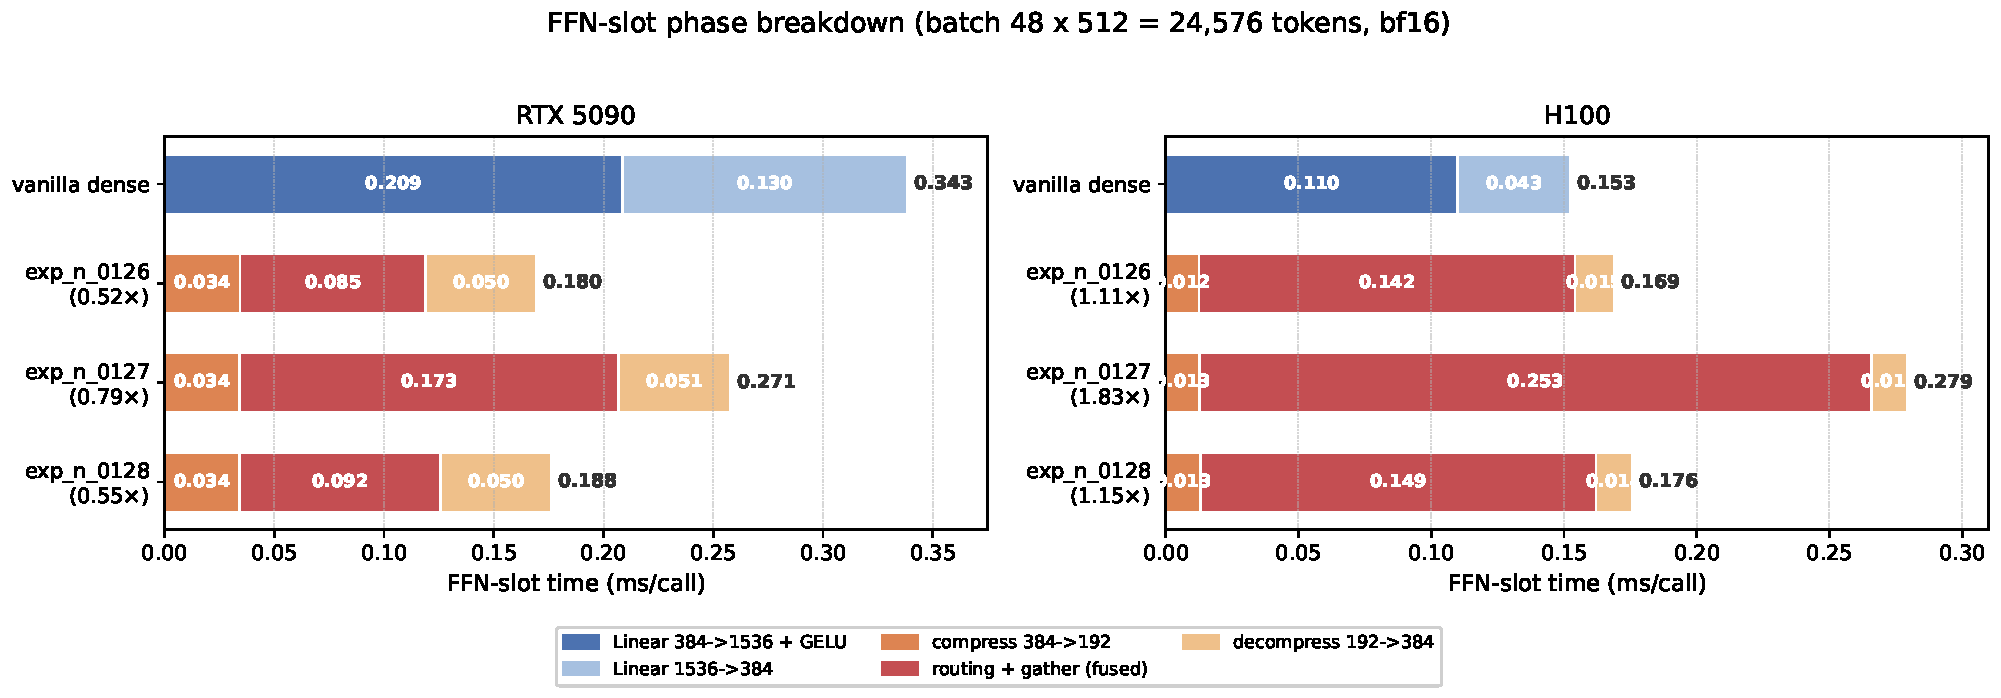
\includegraphics[width=\linewidth]{bench_combined.pdf}
\caption{Per-stage FFN-slot inference time on the two cards (batch $48\times512=24{,}576$ tokens),
left the RTX~5090 and right the H100. The vanilla dense FFN is split into its two matmuls; each
reprojection LUT model is split into compress, fused routing-and-gather, and decompress stages,
with the per-bar total in ms and, for the LUT rows, the LUT/vanilla ratio. On the RTX~5090 (vanilla
$0.343$ ms) the LUT configs run at $0.52$--$0.79\times$ the vanilla time (i.e.\ $1.3$--$1.9\times$
faster); on the H100 (vanilla $0.153$ ms; routed path bf16 compress/decompress with an fp32
bit-exact fused routing-and-gather kernel) they sit slightly \emph{above} the dense baseline
($1.11$--$1.83\times$). On both cards the routing-and-gather stage dominates the LUT cost.}
\label{fig:bench}
\end{figure}

On one stage the two cards trade places. The
fused routing-and-gather, the only part with no matrix multiply, runs $1.5$ to $1.7$
times faster on the RTX~5090 than on the H100, even though the H100 is two to three times faster
on the surrounding dense matmuls and more than twice as fast on the dense FFN overall. The two
operations bind on different hardware. The dense FFN is a tensor-core workload, and the H100 is
built for that. The gather touches no tensor cores; it stays resident in L2 and is bound by SM
clock, and the 5090 clocks its SMs about $1.5$ times higher under load.

We read it as indirect evidence
that the lookup primitive is a distinct kind of workload from dense matrix multiplication, one
worth building specialised hardware for, and that the two already diverge even across shipping
GPUs. Today's accelerators spend their area on
dense-multiply throughput, and there the dense FFN wins. Hardware built for fast gather and large
resident tables would tip the balance.

\clearpage
\section{Conclusion}

A transformer's feed-forward layer can be replaced by a lookup-table family that matches the
dense baseline's bits per byte at a comparable parameter count. The family reprojects the input
into a small subspace, routes it through per-head tables with anchor-pair sign comparisons,
gathers and sums the selected rows, and restores the width with a learned output decompression.
Across the 16k sweep many configurations reach or beat the vanilla bpb while cutting the FFN
block's FLOPs and virtual bandwidth several-fold, at the cost of a larger parameter count.

The match survives longer training. Four 48k-step runs over more than a billion tokens (the
vanilla dense baseline plus three tiny LUT variants) converge shoulder to shoulder; the LUT
finals ($1.15602$, $1.15793$, $1.15962$ bits per byte) sit a hair above the baseline's $1.15144$. A
single representative configuration taken further still, to about $3.5$ billion tokens, likewise
stays within run-to-run noise of the dense baseline.

The deployment picture is hardware-dependent. On an RTX~5090, with hand-written CUDA
kernels, the tiny LUT FFN runs $1.3$ to $1.9$ times faster than the dense FFN at equal quality.
On an H100 the same models are slightly slower, because the H100's dense FFN is extremely fast on
its tensor cores, while the routing-and-gather goes the opposite way and is slower on the H100,
being bound by SM clock rather than tensor cores. The fused kernel narrows the gap for the
smaller configurations but does not overtake it.

We therefore see lookup-table inference as a hardware argument as much as a modelling one. The
lookup-table FFN already matches the dense baseline's quality, and its cost is set by a primitive, reading a
table's selected rows and summing them, that binds on clock and on-chip memory rather than on the
dense-multiply throughput today's accelerators are built to maximise. On current hardware the
dense FFN wins, but the model quality is already in hand and the primitive is simple and regular.
Silicon designed for fast, high-fanout gather and large resident tables would run it at its
natural speed, and would turn parameter storage, the one quantity where the LUT block is heavier,
from a cost into the resource it is built around. That is why we believe the right home for these
models is hardware designed for lookups, and it is the direction we intend to pursue.

\begin{thebibliography}{9}
\bibitem{geva2021} M.~Geva, R.~Schuster, J.~Berant, and O.~Levy.
``Transformer Feed-Forward Layers Are Key-Value Memories.''
\emph{Proceedings of EMNLP}, 2021.
\bibitem{shazeer2017} N.~Shazeer, A.~Mirhoseini, K.~Maziarz, A.~Davis, Q.~Le, G.~Hinton, and
J.~Dean. ``Outrageously Large Neural Networks: The Sparsely-Gated Mixture-of-Experts Layer.''
\emph{ICLR}, 2017.
\bibitem{manifesto} E.~M.~Izhikevich.
``Spiking Manifesto.''
arXiv:2512.11843, December 2025.
\bibitem{nanochat} A.~Karpathy. ``nanochat: a minimal full-stack ChatGPT-style pipeline.''
Software, 2025. \texttt{https://github.com/karpathy/nanochat}.
\bibitem{ltcb} M.~Mahoney. ``Large Text Compression Benchmark.'' Online, 2011.
\texttt{http://mattmahoney.net/dc/text.html}.
\end{thebibliography}

\end{document}
